\input{tuat-common.tex}

\secret{b}{0mm}                 %学外秘/専攻外秘の設定.学部はb(学外秘),修士はm(専攻外秘)にする.
                                %第2引数は位置の調整用.-側に大きくすれば左に寄る.+側に大きくすれば右に寄る.
\pagenum{A-107}%ページ番号 プログラムが確定したら修正を!

\newcommand{\FIGDIR}{./fig}	%図を置くディレクトリを指定する
				%Makefileとは連動していないので注意
\usepackage{pxjahyper} %% これを入れるとしおりが文字化けしない。out2uniが不要になる。
\usepackage{ikuo}%%便利コマンド集.

\hypersetup{
  pdfborder={0 0 0}   % リンクの枠線を無効化
}

\begin{document}
\twocolumn[%
\title{伸縮する棒状ブラキエーションロボットの\\自在移動のための振幅調整法}{Amplitude Adjustment Method for Movement to Arbitrary Locations \\by an Extensible Single-Rod Brachiation Robot}
\author{水内研究室}{大澤 蒼人}{Aoto OSAWA}
\begin{abstract}
  Brachiation is a method of moving by grasping a branch with the upper limbs, and can efficiently move in high places by using gravity. This method is expected to be applied to robots working at heights. In the previous study, using an extensible single-rod brachiation robot, the experimentally determined extending condition was used, so if the target bar positions are different, it need to be determined experimentally again. In this study, we propose an amplitude adjustment method during the pendulum phase of extensible single-rod brachiation robot for brachiation based on bar position.
  And the brachiation movement to arbitrary locations with and without the aerial phase is achieved by using the amplitude adjustment method.
\end{abstract}
\keyword{Brachiation, Excitation, Amplitude adjustment}
]
\begin{small}

\section{緒言}
ブラキエーションは,上肢で枝を掴んでぶら下がりながら移動する方法であり,
重力を利用することで高所を効率的に移動できる.
これをロボットに応用することで\cite{福田敏男1990ブラキエーション形移動ロボットの研究},送電線の点検などの高所作業への応用が期待されている.
従来のブラキエーションロボットはテナガザルを模倣した多リンク型であった.
しかし,多リンク型はカオス現象のような非周期的な運動が発生するため
制御が難しいという問題がある\cite{鈴木三男2000二重振り子におけるカオス的振舞}.
先行研究では,1本の棒状にすることにより問題を解決し,
振子過程でリンクが伸縮する機構を用いてブランコを漕ぐように
振動を拡大させ(これを励振と呼ぶ),適切なタイミングでリンクを伸ばすことで,
同じ高さにある目標バーへの移動を実機で実現した\cite{Hijiri:Robomech2024}.
しかし,この移動は常にグリッパーがバーを把持しており,移動可能距離はロボットの最大長までである.
また,振幅調整は行っておらず,さらにリンクを伸ばすタイミングを実験的に得ているため,目標バーの位置が異なる場合・初期振幅が異なる場合は再度タイミング決定を行わなければならない.
そこで,本研究では目標バーの位置に基づいた振幅調整法を提案し,空中過程無・有の両方のブラキエーション動作タイミングを決定し,
伸縮する棒状ブラキエーションロボットの自在移動を実現させた.

\section{本研究で目的とするブラキエーション動作}
\figref{brachiation}に目的とするブラキエーション動作を示す.
ロボットの両端のグリッパーがそれぞれbar1,bar2を掴んだ状態(\figref{brachiation}(1))から,
bar1を離して振子過程(\figref{brachiation}(2))に移る.
bar3がロボットの伸縮可能最大長以下の距離にある場合,リンクを伸ばすことで空中過程を含まずに移動する(\figref{brachiation}(3‐1)).
bar3が伸縮可能最大長より離れている場合,適切なタイミングでbar2を離し(\figref{brachiation}(3‐2)),
空中過程を経てbar3を掴む(\figref{brachiation}(4)).この一連の流れを繰り返すことにより,bar3以降も連続してブラキエーションをすることができる.

ここで,先行研究ではリンクを伸ばすタイミング,bar2を離すタイミングを実験的に決定していたため,バーが異なる位置にある場合や連続ブラキエーションにより初期振幅がずれた場合,ブラキエーション動作の継続が困難となる.
空中過程を含まない場合は,目標バーを把持するために必要な振幅まで励振し,
空中過程を含む場合は,適切なリリース条件になるための振幅まで励振することが望まれる.
そこで,本研究では振子過程で振幅を調整することで,バーの位置に基づいたブラキエーション動作を目指した.

\section{伸縮量制御による振幅調整法}
\subsection{振幅に基づくロボット最大長の決定}
伸縮する機構を活かし,励振時のロボット最大長$l_{\mathrm{max}}$を変えることで振幅増加率を変化させることができる.
本研究では振子過程において半周期ごとに現在振幅と目標振幅から振幅増加率を求め,ロボット最大長を決定する.
ここで,ロボットを長さ可変の一本の剛体棒であるとみなすと,運動方程式は角度$\varphi$,長さ$l$,質量$m$,回転軸周りの慣性モーメント$J$,重力加速度$g$,減衰係数$c$を用いて
\equref{equation}で表される.
\begin{eqnarray}
  \equlabel{equation}
  J \frac{\mathrm{d}^2 \varphi}{\mathrm{d} t^2} +c \frac{\mathrm{d}\varphi}{\mathrm{d} t}+\frac{1}{2}mgl \sin{(\varphi)}=0
\end{eqnarray}
しかし,\equref{equation}は非線形な項を含むため,振動の振幅が微小である($\sin{(\varphi)}\approx \varphi$)とみなした近似\equref{Approximation Model}
でのモデル化を試みた.
なお,角振動数を$\omega$とし,本研究において初期位相は$\phi=0$とした.
これにより,現在振幅$A_{\mathrm{now}}$から半周期後に目標振幅$A_{\mathrm{ref}}$になるために必要な振幅増加率$\lambda$は\equref{lambda}で表せる.
\begin{eqnarray}
  \equlabel{Approximation Model}
  \varphi(t)&=&A_{\mathrm{now}}e^{\lambda t}\cos{(\omega t + \phi)}\\
  \equlabel{lambda}
            \lambda&=&\frac{\omega}{\pi}\ln{\left(\frac{A_{\mathrm{ref}}}{A_{\mathrm{now}}}\right)}
\end{eqnarray}
ここで,微小角近似ができない振幅になると周期は振幅に依存するため,実験データより振幅$A$と角振動数$\omega$の関係を
$\omega=-0.0126A+4.64$と近似した.
これらを基に,ロボット最大長$l_{\mathrm{max}}$が異なる実験データごとに振幅増加率を調整し,
フィッティングした.フィッティング結果のうち$l_{\mathrm{max}}=$0.74, 0.68mの結果を\figref{Fitting}に示す.
これにより,ロボット最大長と振幅増加率の関係は$l_{\mathrm{max}}=0.99\lambda+0.60$と近似された.
以上により,現在振幅$A_{\mathrm{now}}$から半周期後に目標振幅$A_{\mathrm{ref}}$にするためには次式を用いて求めることができる.
\begin{eqnarray}
  \equlabel{l status}
  l_{\mathrm{max}}=\frac{0.99(-0.0126A_{\mathrm{now}}+4.64)}{\pi}\ln{\left(\frac{A_{\mathrm{ref}}}{A_{\mathrm{now}}}\right)}+0.60 \nonumber
\end{eqnarray}
\subsection{振幅調整実験}
目標振幅を負の角度範囲で$A_{\mathrm{ref}}=$120 degとし,振幅調整実験を行った.
角度変化とロボット最大長指令値を\figref{Adjust}に示す.黒線は目標振幅,赤線は目標振幅到達時刻を表す.
なお,ロボット最大長はリンク伸縮可能範囲内($0.56\mathrm{m}\le l_{\mathrm{max}} \le 0.74\mathrm{m}$)で半周期ごとに決定した.
これにより伸縮量制御による振幅調整法の有用性を確認した.
%% \clearpage

\section{空中過程を含まないブラキエーション動作実験}
提案した振幅調整法を用いて空中過程を含まないブラキエーション動作実験を行った.
目標バー把持直前の半周期は励振動作のない単純な減衰とし,ロボット長はバーまでの距離を基に決定した.
最後の半周期での減衰を考慮した目標振幅を求め,振幅調整を行った.
実験の様子を\figref{NoAerial}に示す.なお,実験1は同じ高さ,実験2は異なる高さに目標バーを設置した.
成功率はいずれの位置のバーでも50%程であった.


% \clearpage
\begin{figure*}[t]
  \centering
  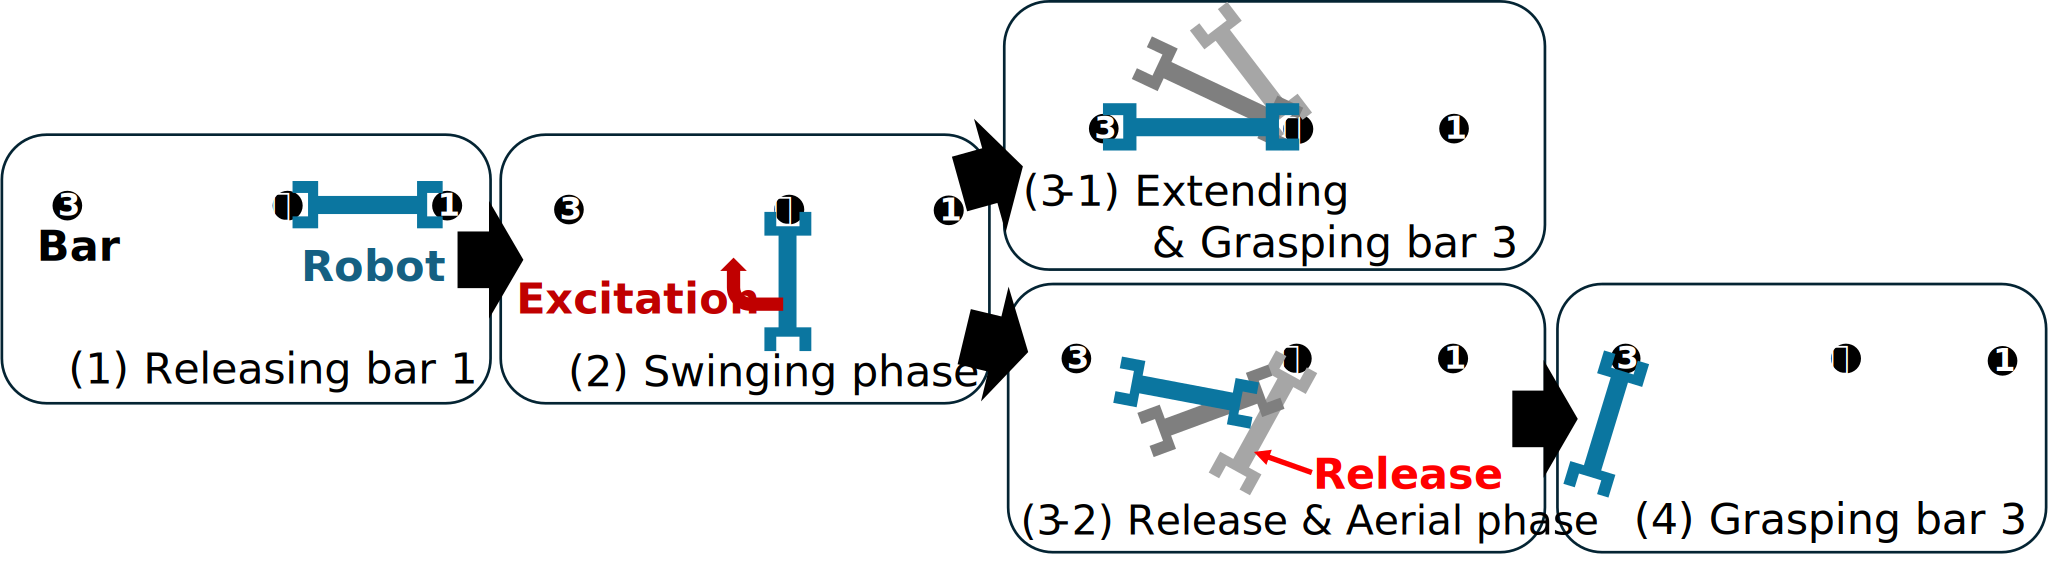
\includegraphics[width=0.7\textwidth]{fig/brachiationFig-4.eps} % 画像のパスを指定
  \vspace{-5mm}
  \caption{Brachiation motions}
  \figlabel{brachiation}
\end{figure*}
\begin{figure}[t]
  \centering
  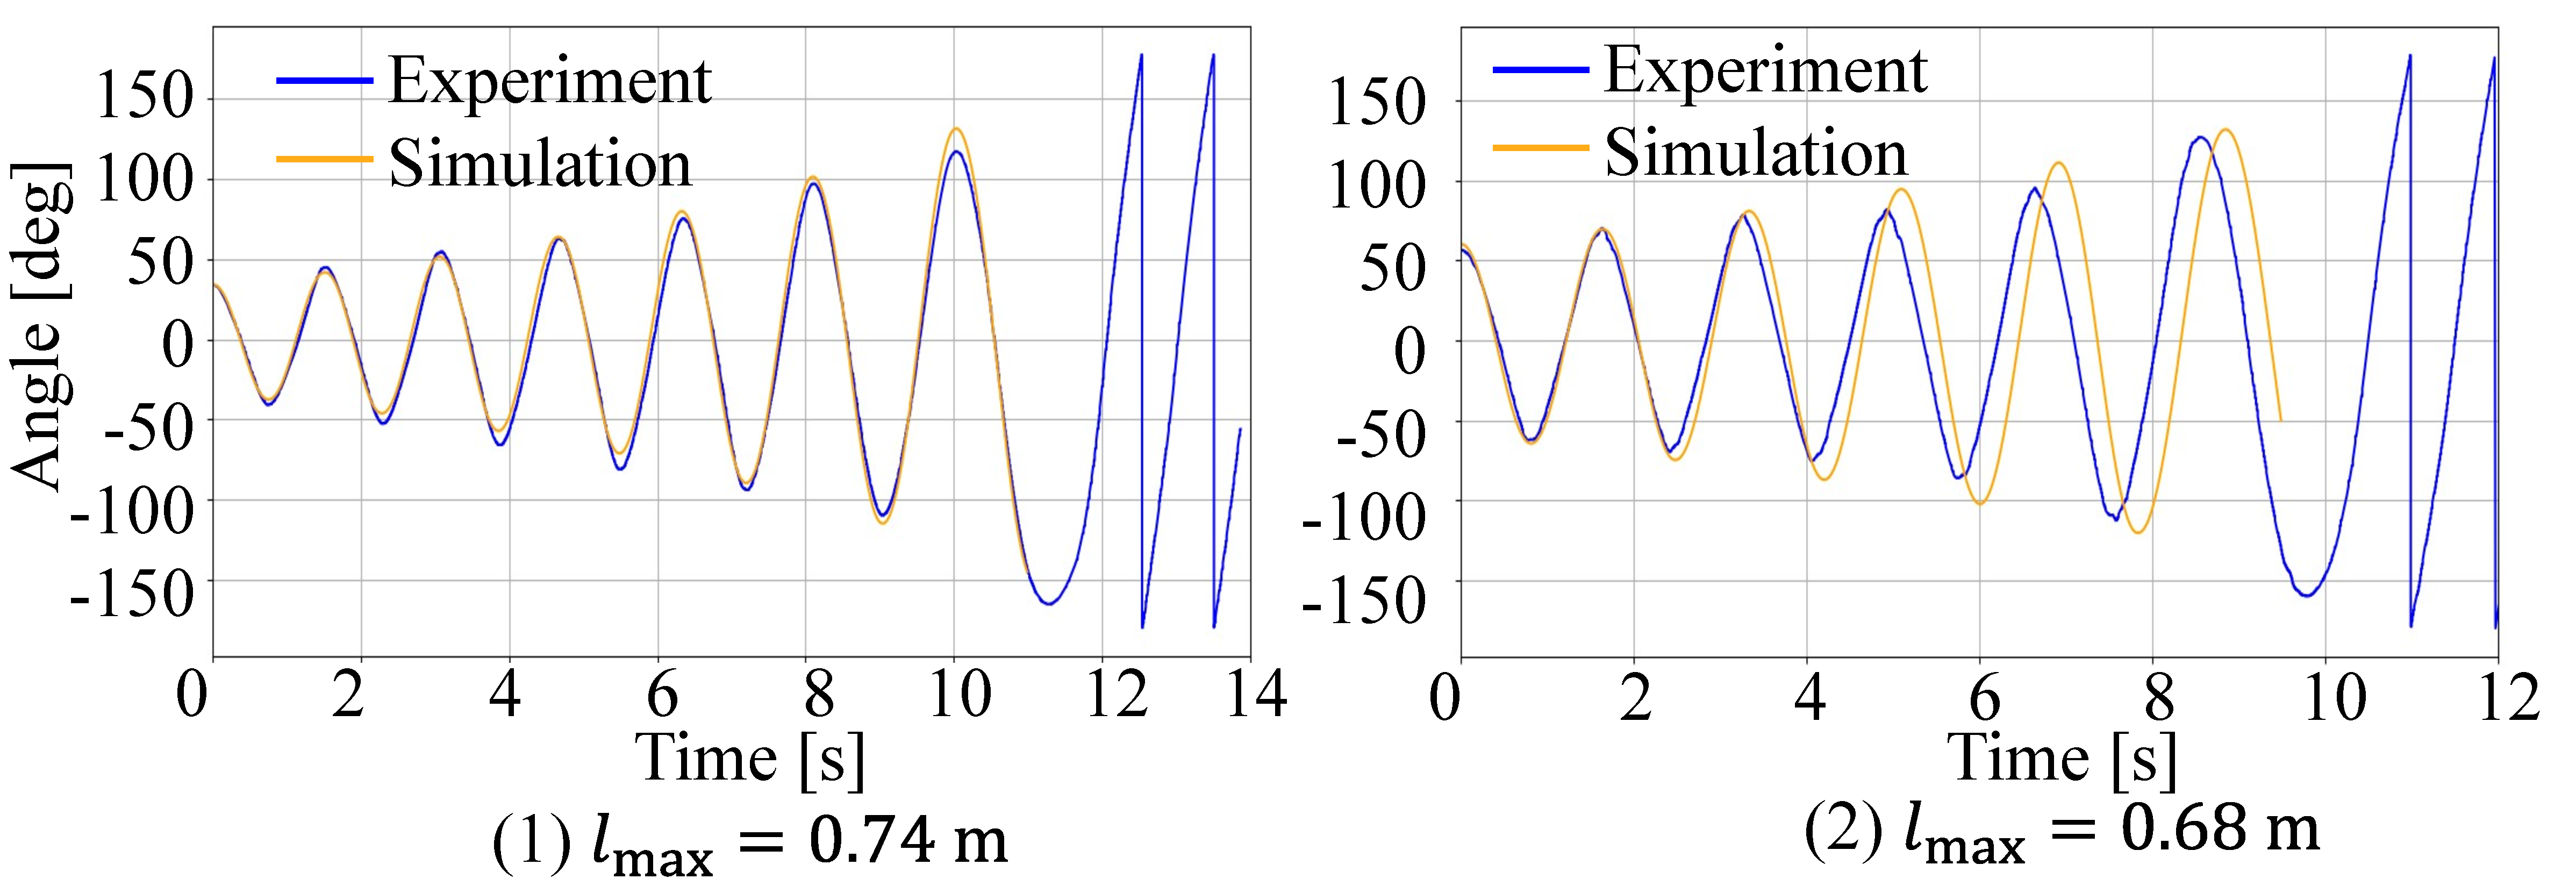
\includegraphics[width=0.53\textwidth]{fig/FittingAngle3.eps} % 画像のパスを指定
  \vspace{-10mm}
  \caption{Fitting results of angle($l_{\mathrm{max}}=$0.74, 0.68m)}
  \figlabel{Fitting}
\end{figure}
\begin{figure}[h]
  \centering
  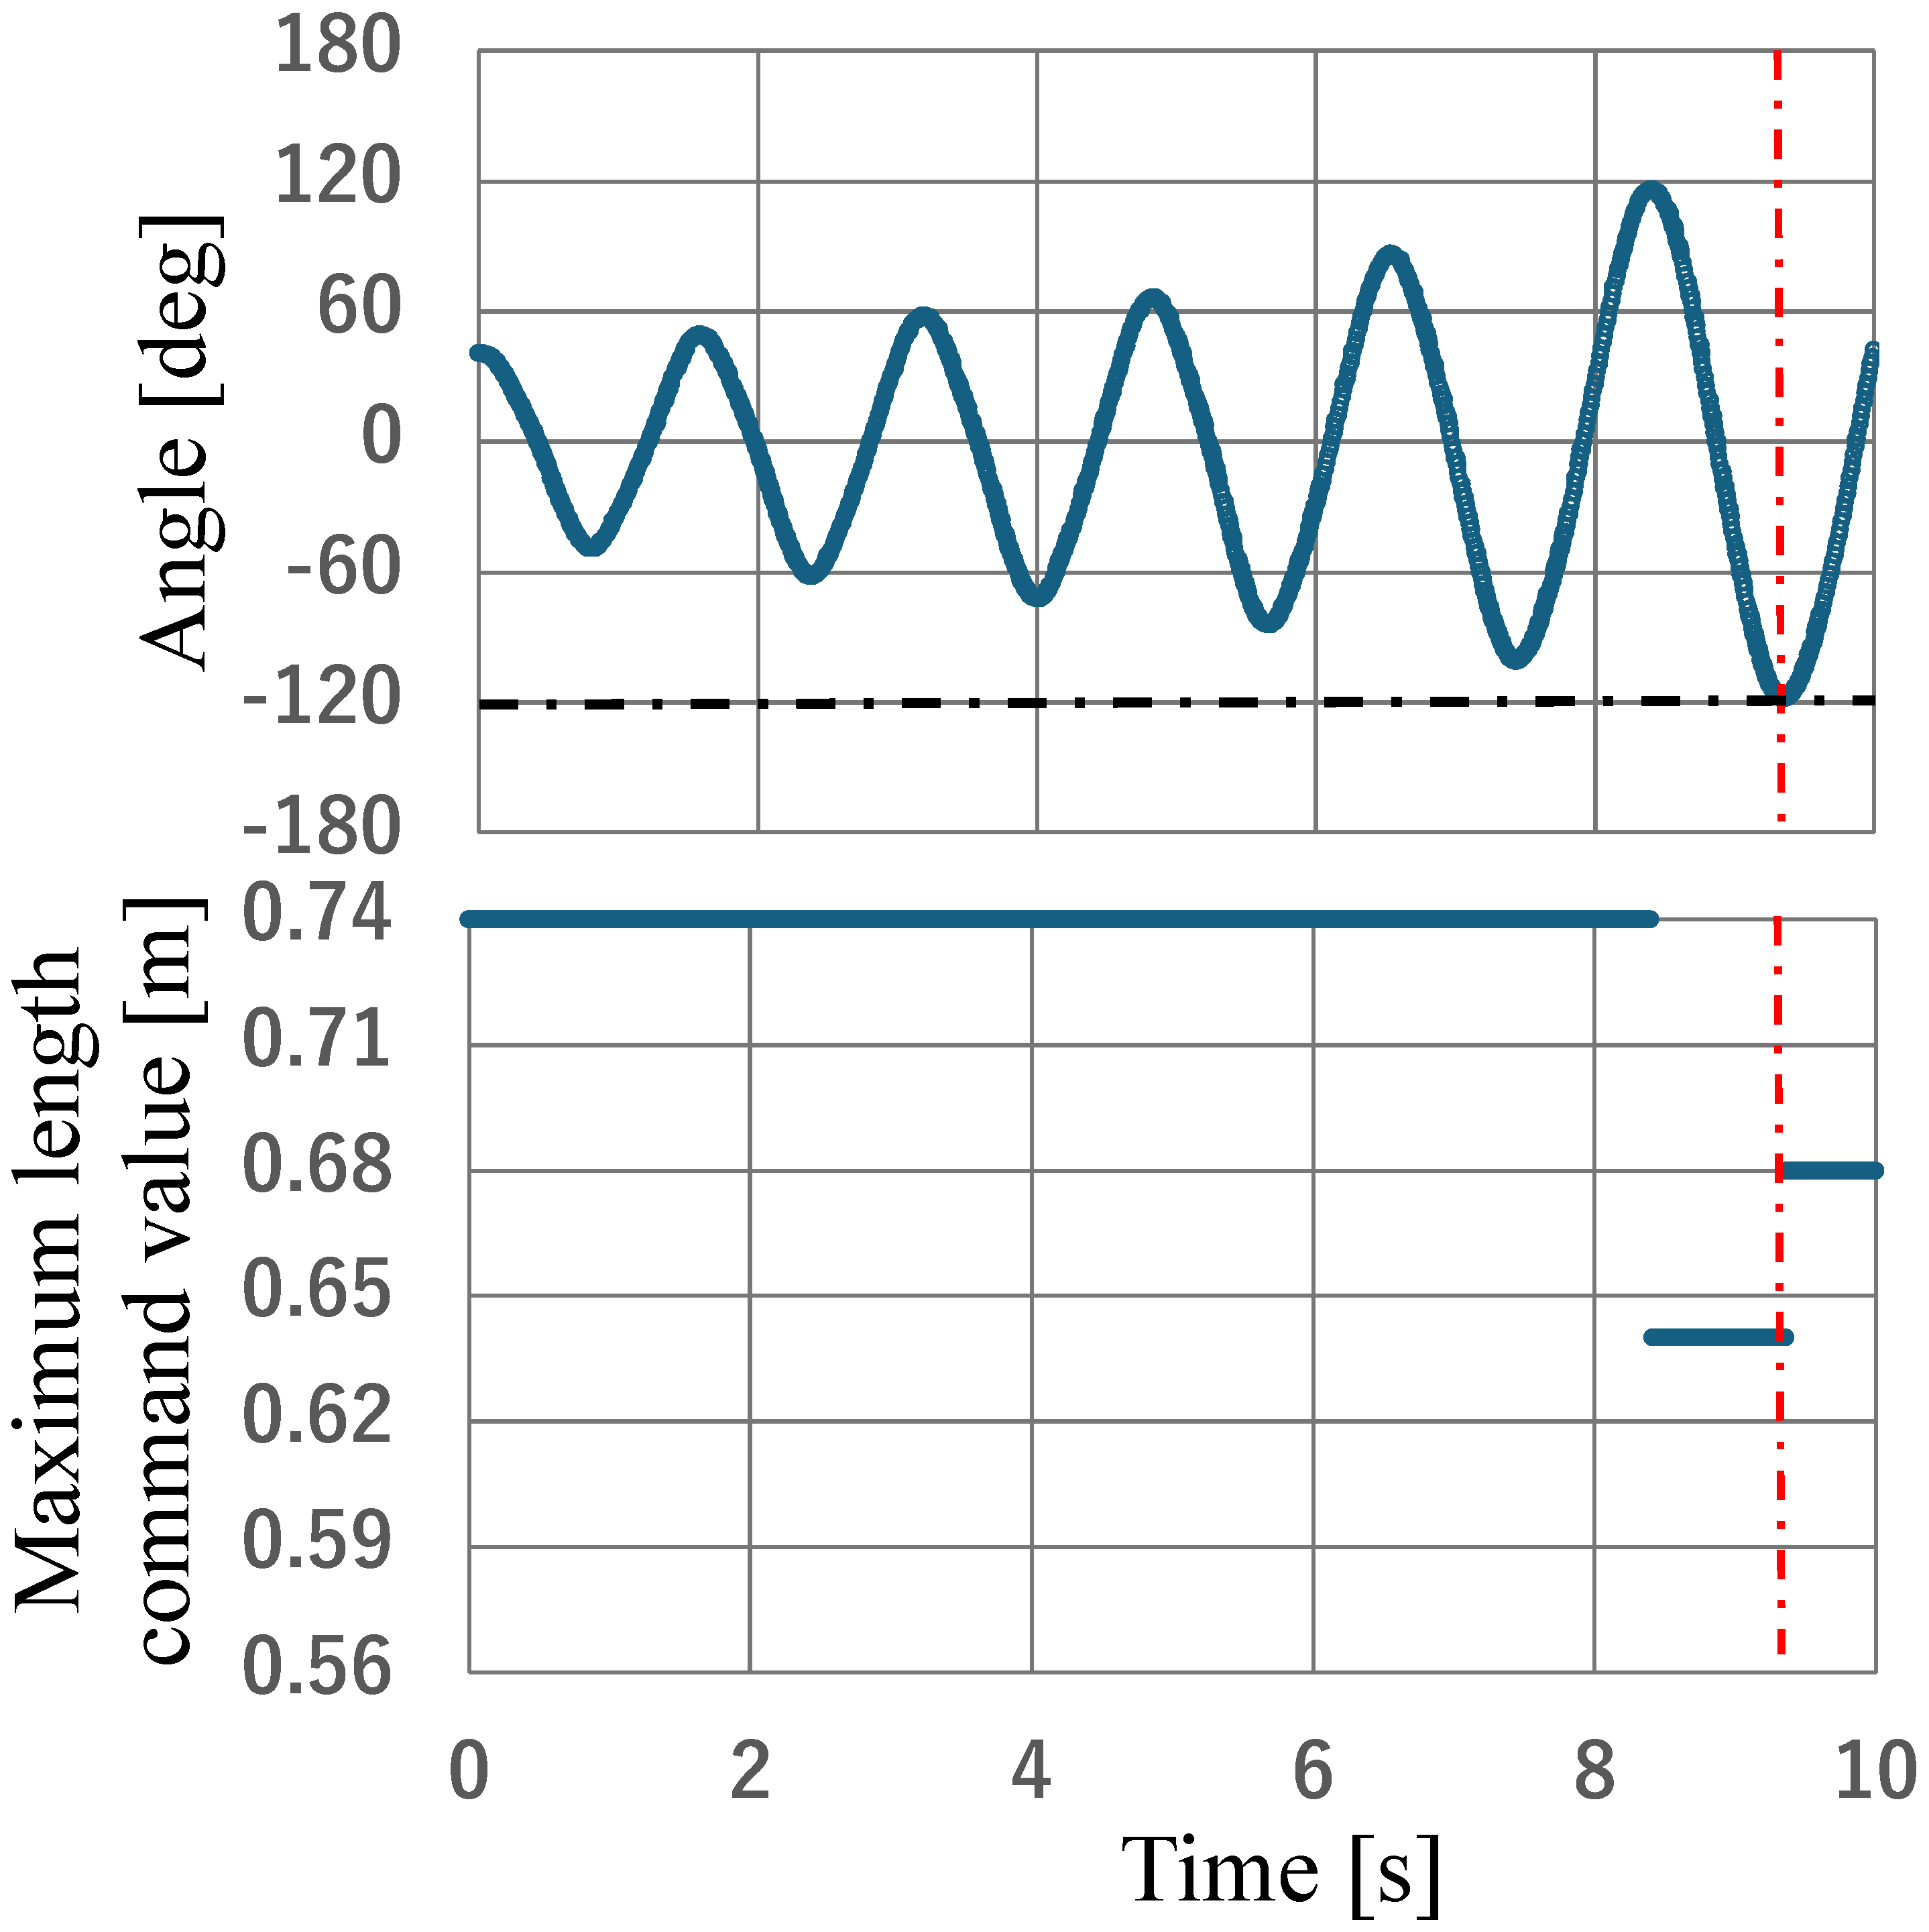
\includegraphics[width=0.3\textwidth]{fig/AdjustForMaezuri.eps} % 画像のパスを指定
  \vspace{-7mm}
  \caption{Amplitude adjustment experiment}
  \figlabel{Adjust}
\end{figure}
\begin{figure}[t]
  \centering
  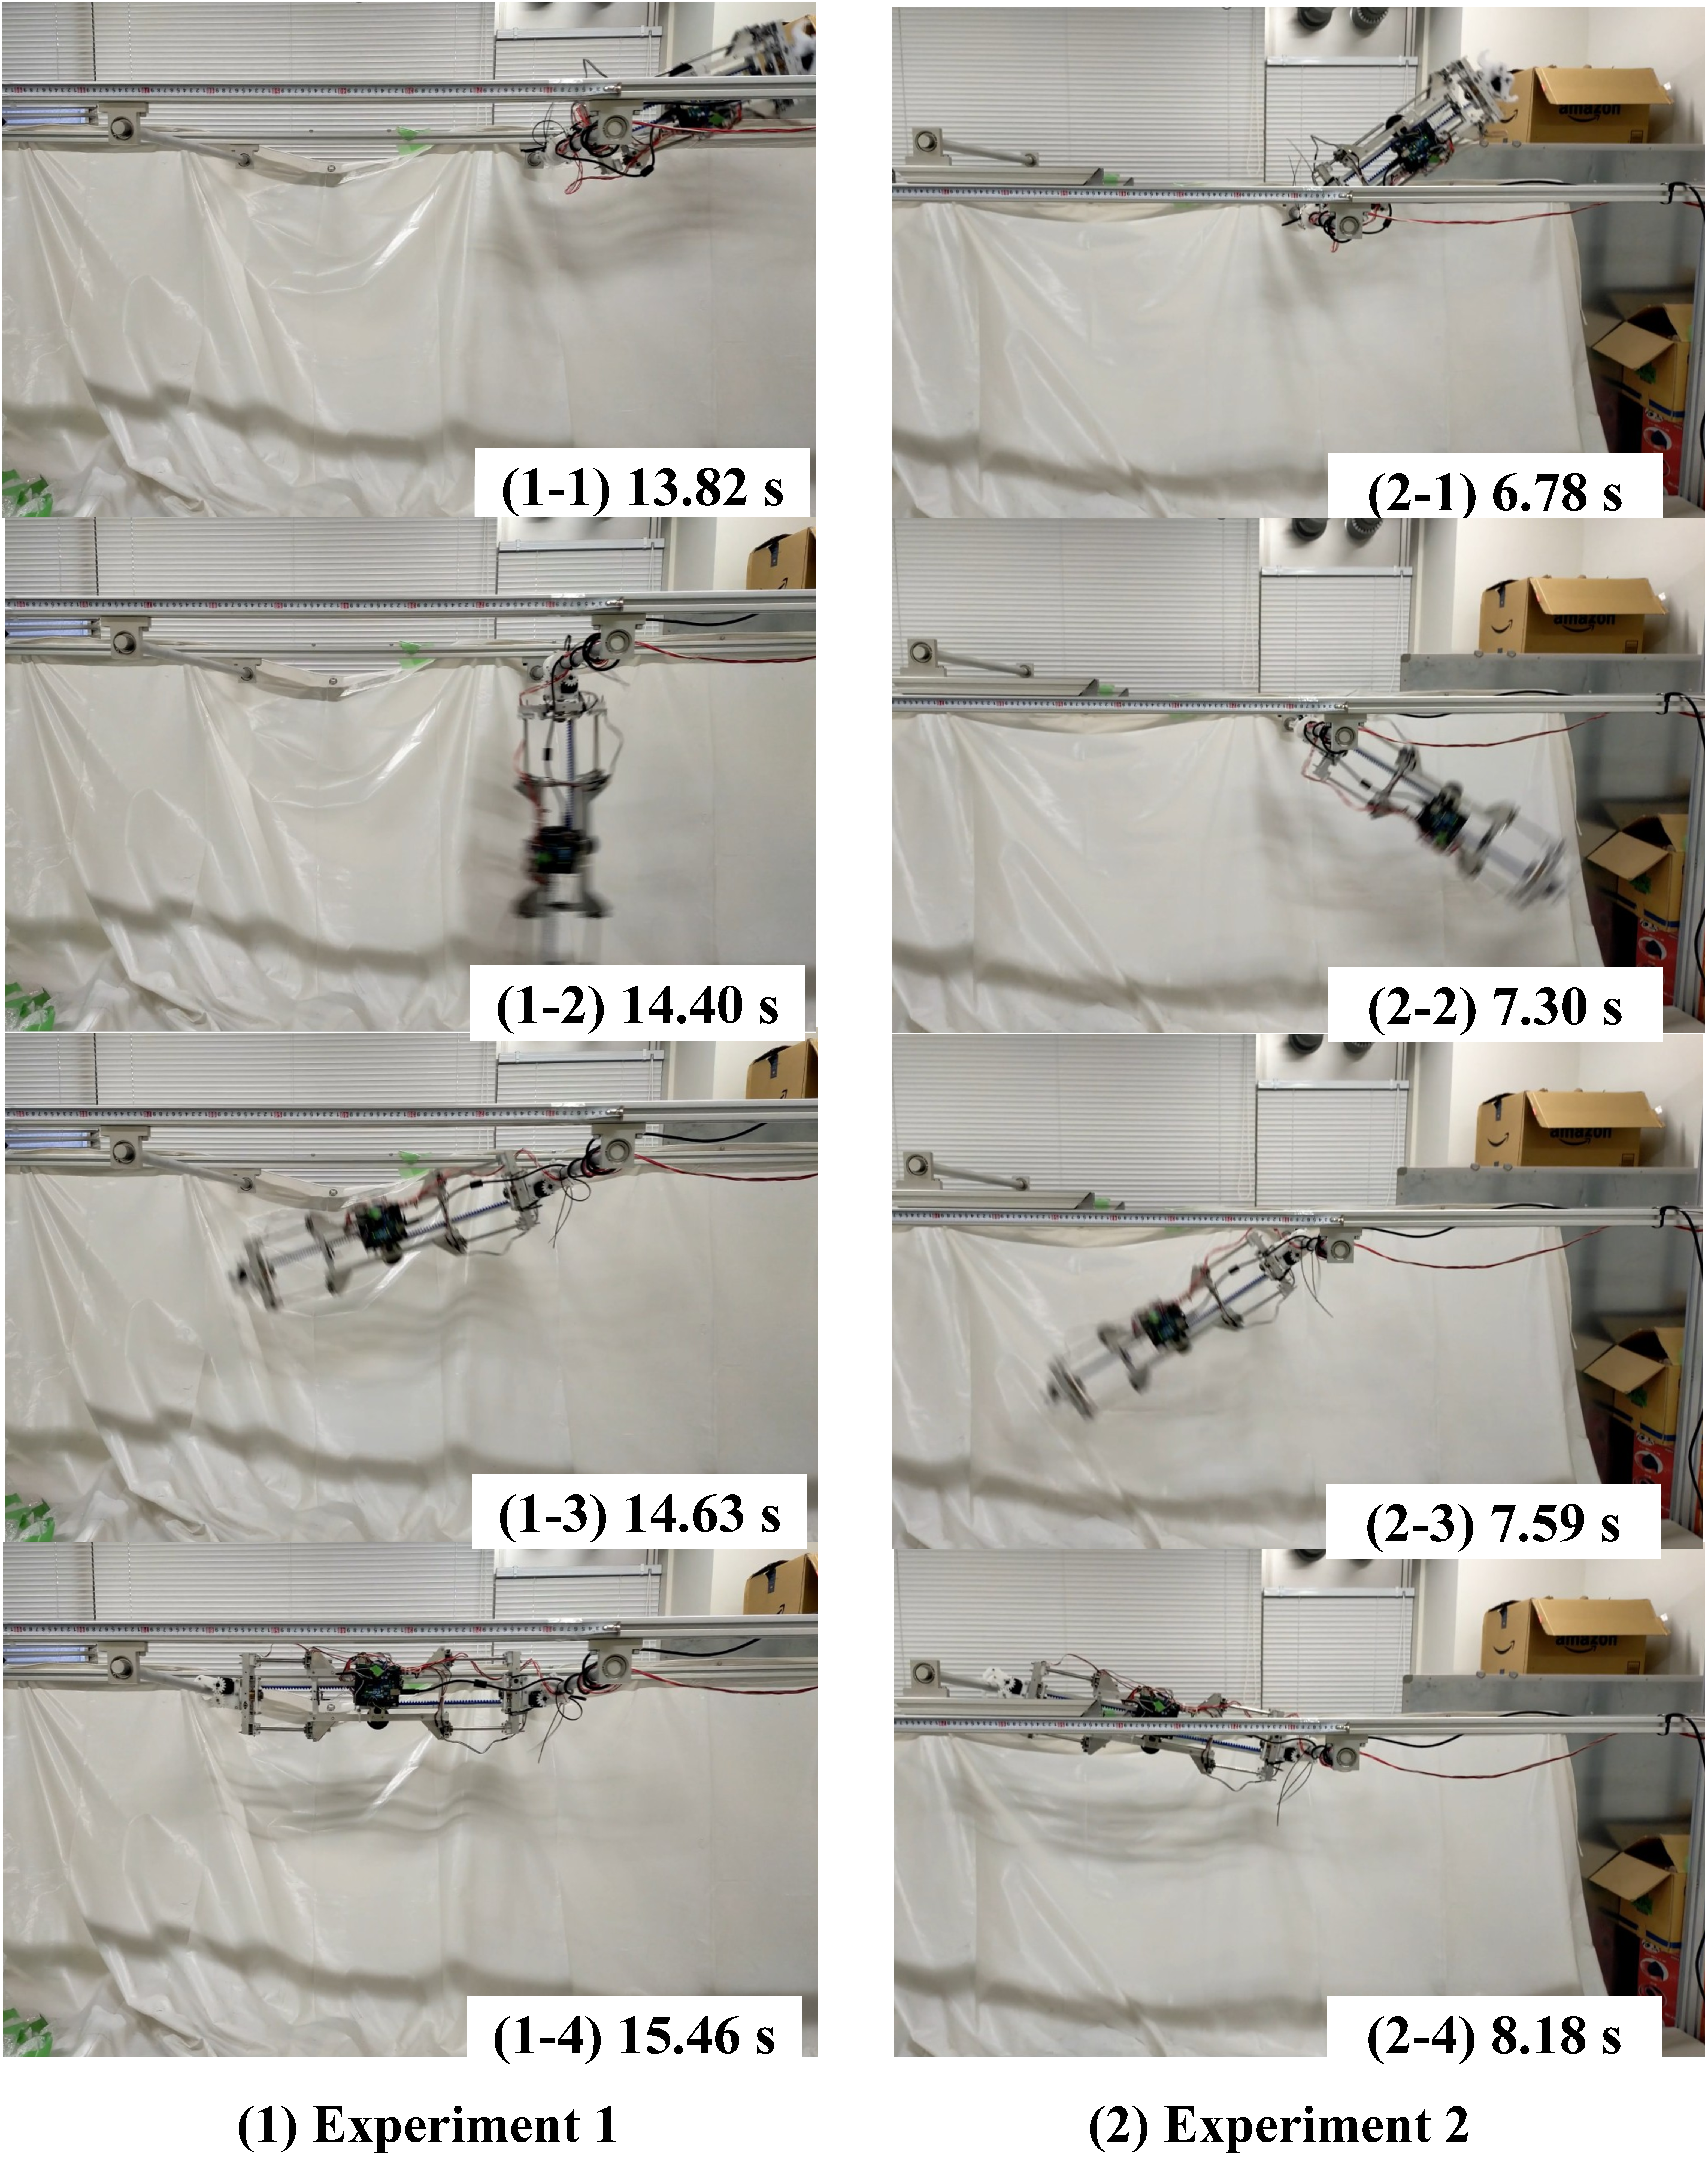
\includegraphics[width=0.4\textwidth]{fig/NoAerialForMaezuri.eps} % 画像のパスを指定
  \vspace{-5mm}
  \caption{No aerial phase experiment}
  \figlabel{NoAerial}
\end{figure}
\begin{figure}[t]
  \centering
  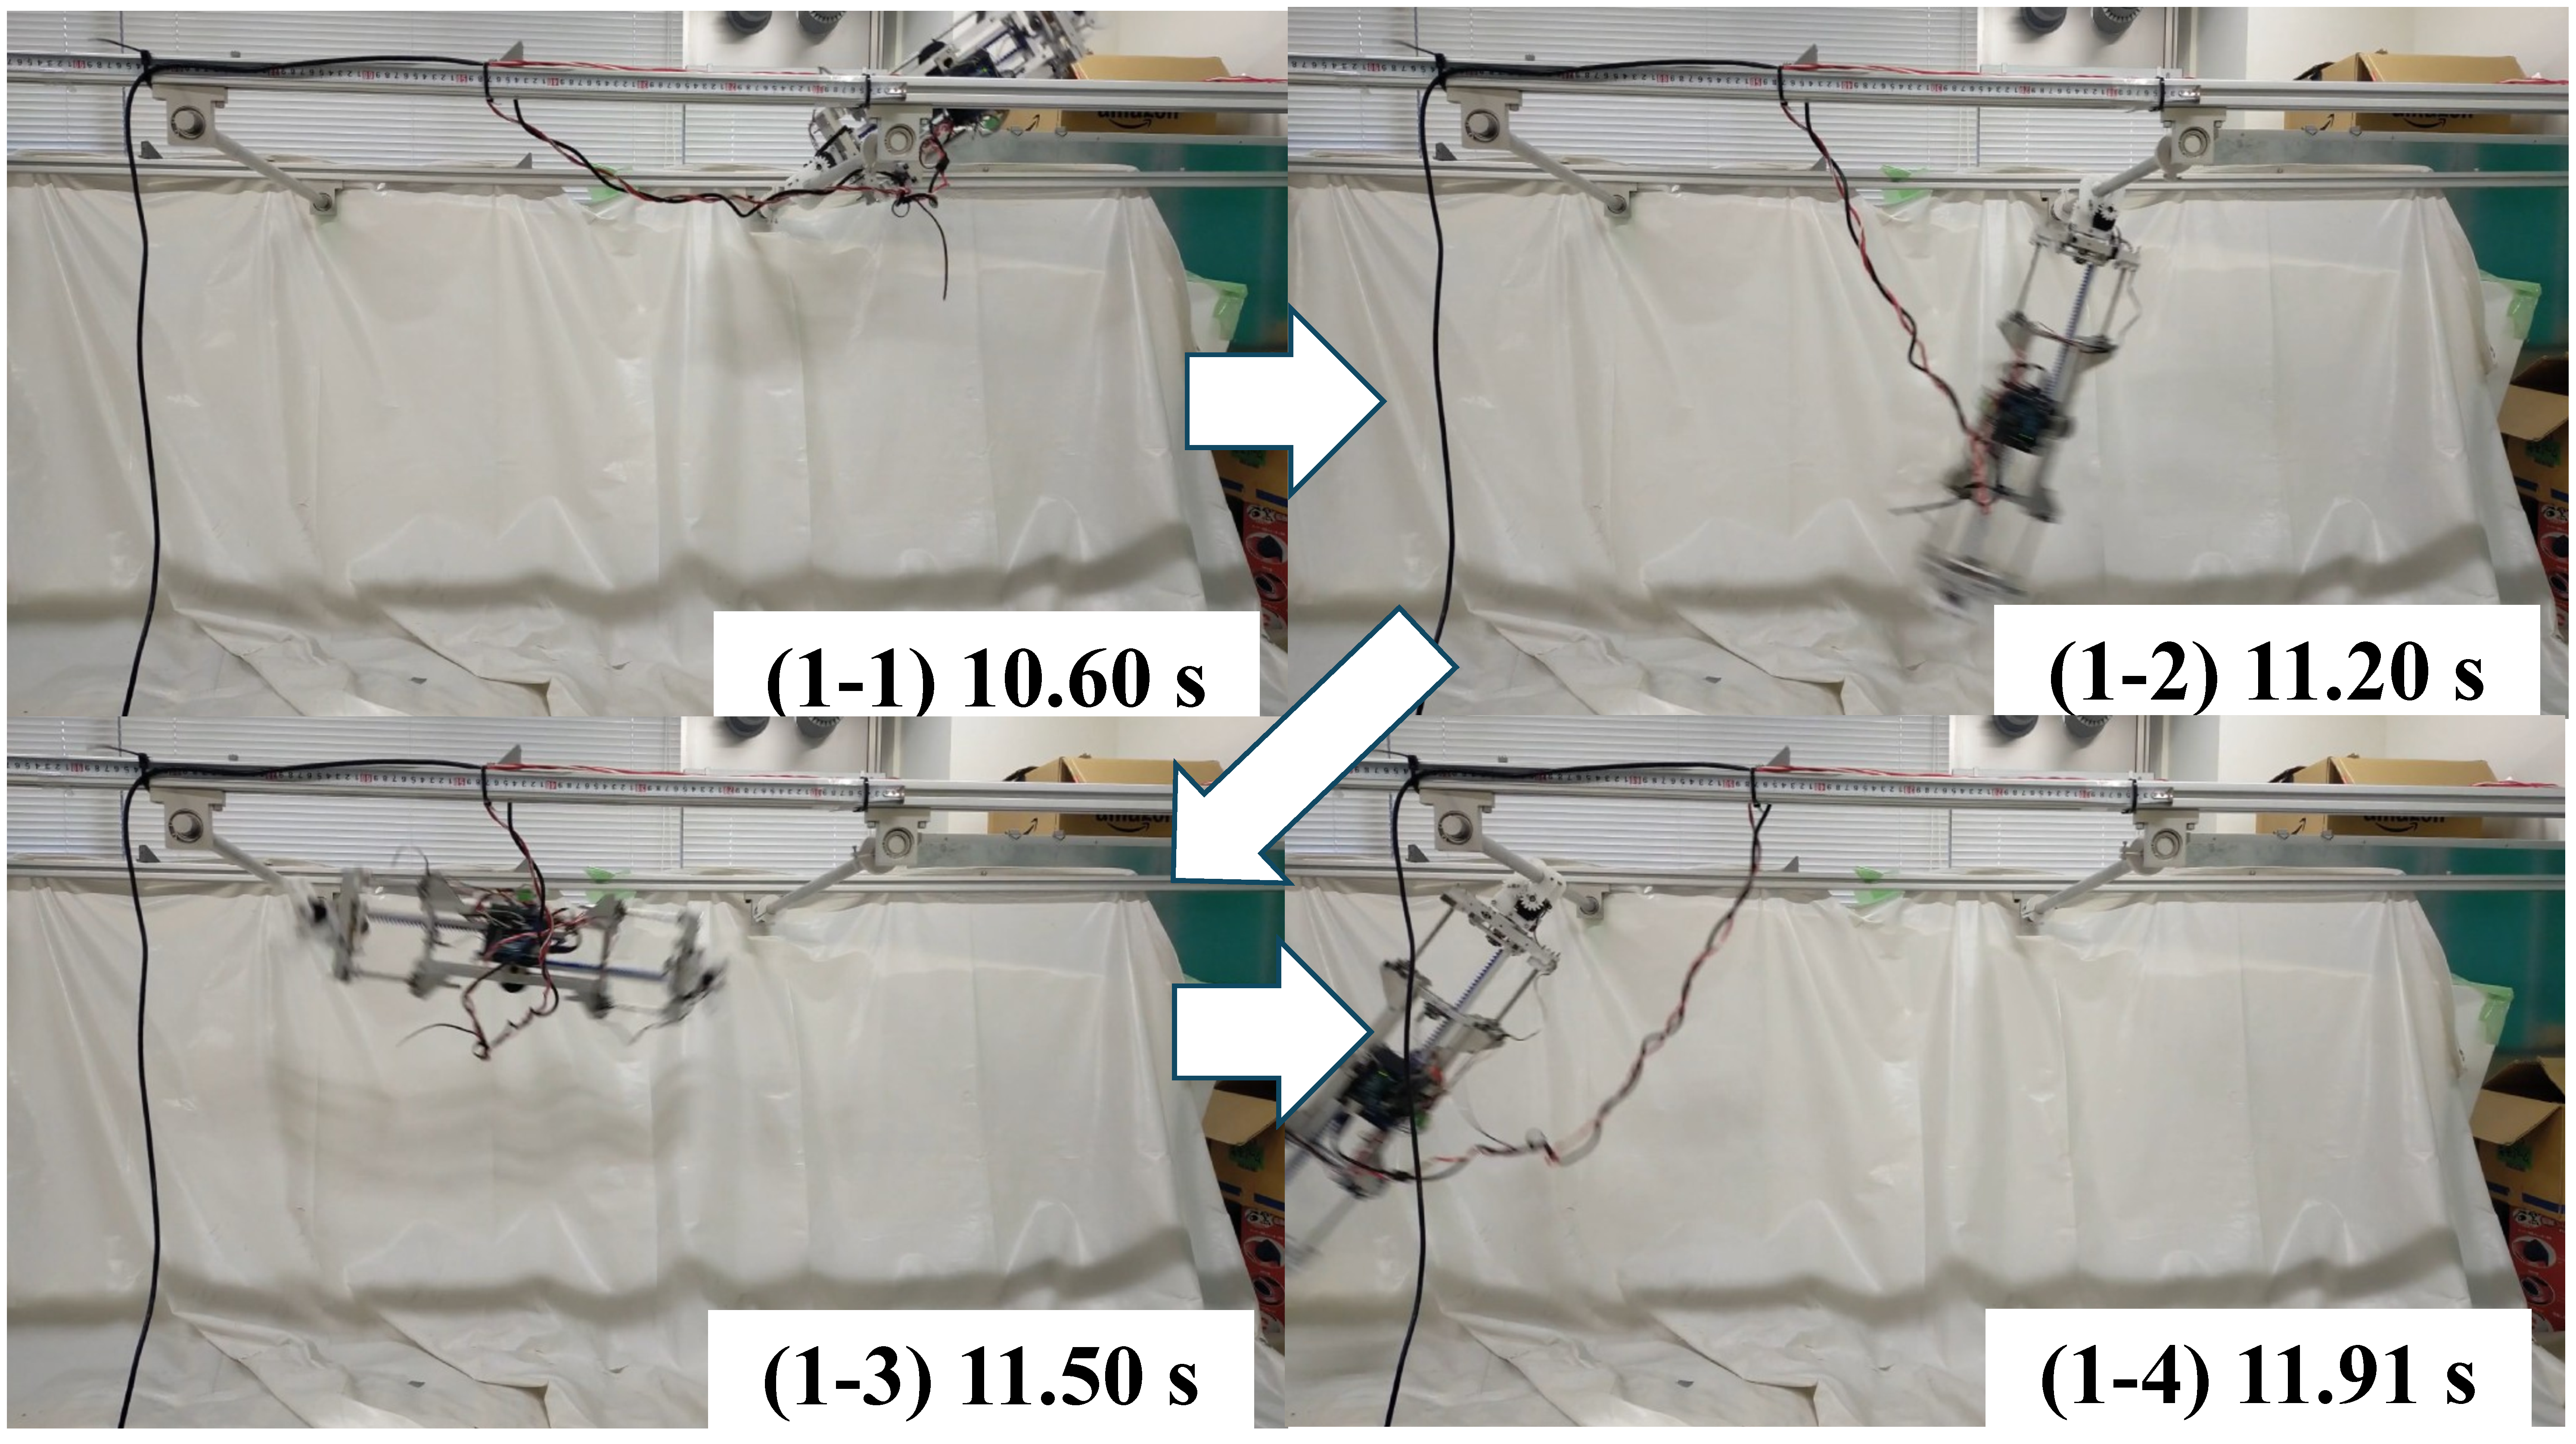
\includegraphics[width=0.4\textwidth]{fig/AerialForMaezuri.eps} % 画像のパスを指定
  \vspace{-5mm}
  \caption{Aerial phase experiment}
  \figlabel{Aerial}
\end{figure}
\section{空中過程を含むブラキエーション動作実験}
提案した振幅調整法を用いて空中過程を含まないブラキエーション動作を行った.
なお,バーリリース後のロボット長を一定とすることで空中過程では重心は放物線軌道,グリッパーはリリース時の角速度による重心周りの一定速回転軌道となる.
目標バーを,もともと把持しているバーと同じ高さでロボット伸縮可能最大長さ0.74mから50cm離れた位置に設置した.
安定したバー把持を行うために,バー把持時のバーとグリッパーの距離$J_{\mathrm{d}}$・バーに対するグリッパーの加速度$J_{\mathrm{r}}$を基に,
距離に重み付け($\alpha$)を行った評価関数$J=\alpha \times J_{\mathrm{d}}+J_{\mathrm{r}}$を定義し,
$J$を最小とするリリース時角度・角速度・ロボット長を最適なバーリリース条件とした.
その条件になるように,単純減衰であるとして必要な目標振幅を求め,振幅調整を行った.
実験の様子を\figref{Aerial}に示す.成功率は6.7%程とかなり低かった.その原因として,バー把持時のグリッパー角度が挙げられる.
グリッパーの構造上,振子の回転軸方向に振動が発生してしまうため,バーに対して垂直にリリースされない場合がある.
回転軸方向に振動が発生しにくい構造にすることでより安定した把持が可能となり,成功率増加が期待できる.
\section{結言}
伸縮する棒状ブラキエーションロボットの伸縮量制御による振幅調整法を提案した.
また,目標バーの位置に基づいてブラキエーション動作計画を決定し,その計画を振幅調整法によって実現させ,
空中過程無・有の両方のブラキエーションに成功させ,自在移動を達成した.

%% \begin{thebibliography}{99}
%% \small
%%  \setlength{\kanjiskip}{0.0zw plus.01zw} %
%%  \setlength{\baselineskip}{9pt}        %
%%  \setlength{\itemsep}{0.2pt}             %
%%  \setlength{\lineskip}{0pt}              %
%%  \setlength{\normallineskip}{0.2pt}      %


%% \bibitem{hogege} 川村マサキ,
%% ほげの可能性と適用限界に関する実験的研究,日本ほげ学会ほげ工学部門講演会,(2010).


%% \bibitem{hohoge} 本堂貴敏,
%% ほげの力学,(2006),pp.11--43,ほげ出版.

%% \end{thebibliography}

{
%% \scriptsize %%←どうしても入らない時は,このコメントをはずすと少し小さくなる.
\bibliographystyle{junsrt}
\bibliography{reference}
}

\end{small}
\end{document}
